\documentclass[tikz,border=5mm]{standalone}
\usetikzlibrary{arrows.meta,calc}

\begin{document}
	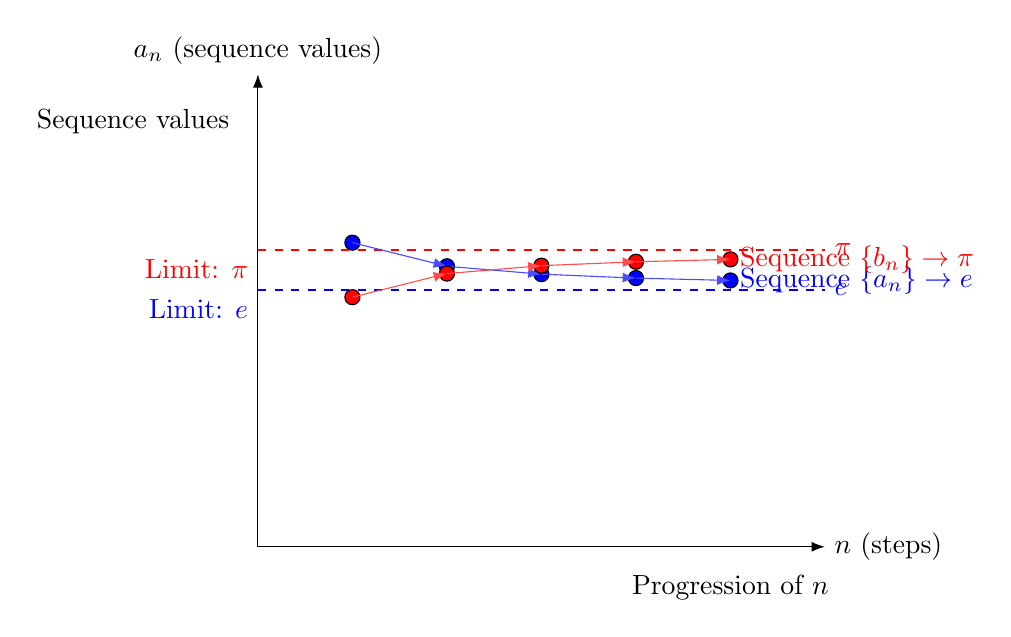
\begin{tikzpicture}[scale=1.2, >=Latex]
		% Axes
		\draw[->] (0,0) -- (6,0) node[right] {$n$ (steps)};
		\draw[->] (0,0) -- (0,5) node[above] {$a_n$ (sequence values)};
		
		% Sequence 1: Converging to e
		\foreach \n in {1,2,3,4,5} {
			\coordinate (a\n) at (\n, {2.718+0.5/\n});
			\draw[fill=blue] (a\n) circle (0.08);
		}
		\draw[dashed, blue] (0,2.718) -- (6,2.718) node[right] {$e$};
		\node[blue, right] at (a5) {Sequence $\{a_n\} \to e$};
		
		% Arrows for Sequence 1
		\foreach \n in {1,2,3,4} {
			\pgfmathtruncatemacro{\m}{\n+1}
			\draw[->, blue!70] (a\n) -- (a\m);
		}
		
		% Sequence 2: Converging to pi
		\foreach \n in {1,2,3,4,5} {
			\coordinate (b\n) at (\n, {3.141-0.5/\n});
			\draw[fill=red] (b\n) circle (0.08);
		}
		\draw[dashed, red] (0,3.141) -- (6,3.141) node[right] {$\pi$};
		\node[red, right] at (b5) {Sequence $\{b_n\} \to \pi$};
		
		% Arrows for Sequence 2
		\foreach \n in {1,2,3,4} {
			\pgfmathtruncatemacro{\m}{\n+1}
			\draw[->, red!70] (b\n) -- (b\m);
		}
		
		% Legends
		\node[below left, blue] at (0,2.718) {Limit: $e$};
		\node[below left, red] at (0,3.141) {Limit: $\pi$};
		
		% Additional labels
		\node[below] at (5,-0.2) {Progression of $n$};
		\node[left] at (-0.2,4.5) {Sequence values};
		
	\end{tikzpicture}
\end{document}
